\documentclass[a4paper, 16pt]{article}
\usepackage[english]{babel}
\usepackage[utf8]{inputenc}
\usepackage[T1]{fontenc}
\usepackage{lmodern}
\usepackage{multirow}
\usepackage{graphicx}
\usepackage{amsmath}
\usepackage{amssymb}
\usepackage{amsfonts}
\usepackage{graphicx}
\usepackage{chngpage}
\usepackage{pythonhighlight}

\usepackage{float}
\usepackage[caption = false]{subfig}

\graphicspath{{figures/}}


\title{%
    Solving PDE\\ 
    \large Report}
\date{2022\\ November}
\author{Zala Stopar Špringer}

\begin{document}

\maketitle
\pagenumbering{gobble}


\newpage

\tableofcontents

\newpage
\pagenumbering{arabic}

\section{$x \in [0 100], hx = 5 and y \in [-50, 50], hy = 1$}

\subsection{Heatmap}


\begin{figure}[H]
\subfloat[0-3]{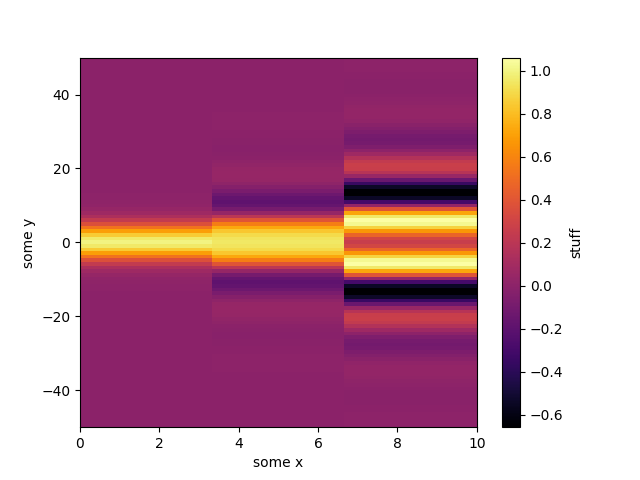
\includegraphics[width = 0.7\textwidth]{../plots/heatmap0-3.png}}
\subfloat[0-5]{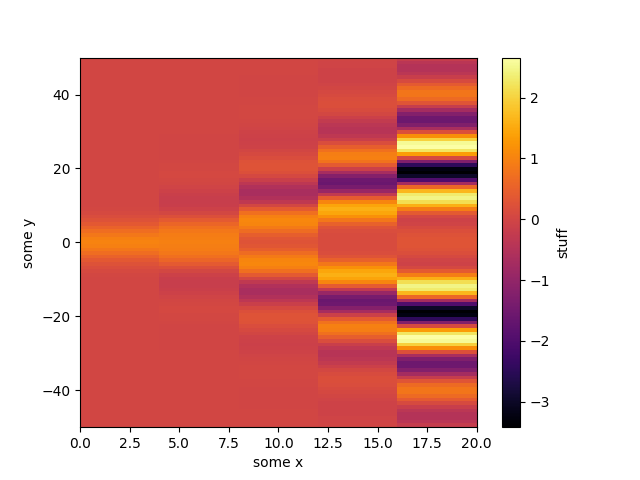
\includegraphics[width = 0.7\textwidth]{../plots/heatmap0-5.png}} \\
\subfloat[0-10]{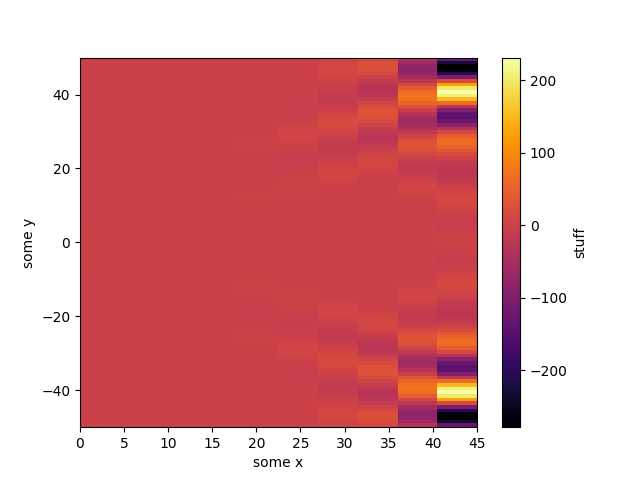
\includegraphics[width = 0.7\textwidth]{../plots/heatmap0-10.png}}
\subfloat[0-20]{{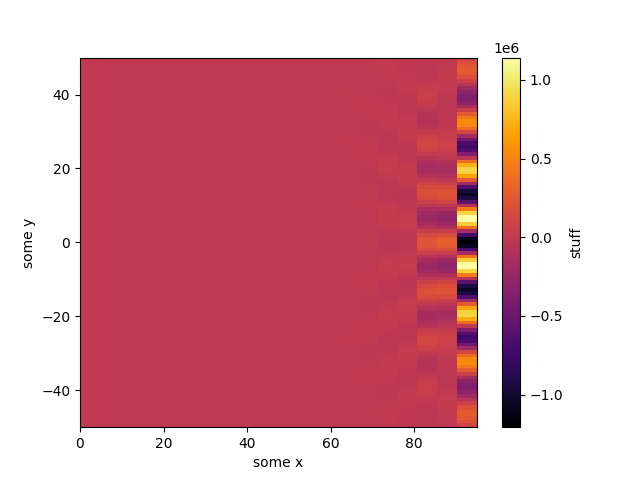
\includegraphics[width = 0.7\textwidth]{../plots/heatmap0-20.png}}
}
\caption{Heatmap for first n x numerically calculated}
\label{some example3}
\end{figure}



    \begin{figure}[!h]
        \makebox[\textwidth]{
        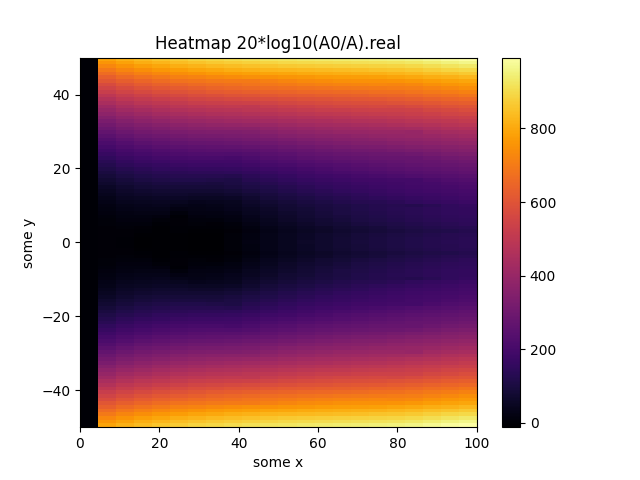
\includegraphics[width = 0.7\textwidth]{../plots/decibels.png}}
¸    \caption{numerical solution}
        \label{fig: napaka}
    \end{figure}


    \begin{figure}[!h]
        \makebox[\textwidth]{
        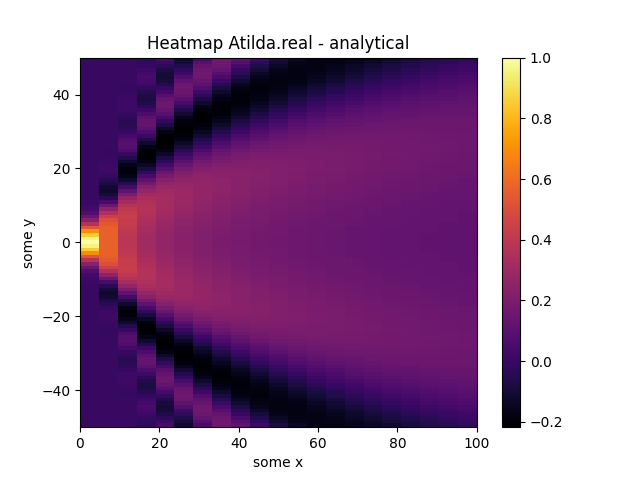
\includegraphics[width = 0.7\textwidth]{../plots/heatmap_tilda.png}}
¸    \caption{analytical solution}
        \label{fig: heatana}
    \end{figure}

\newpage

\subsection{Compare numerical and analytical}


\begin{figure}[H]
\subfloat[x=0]{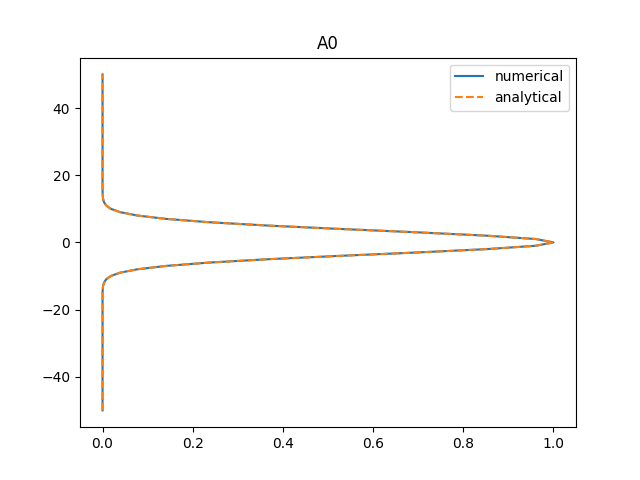
\includegraphics[width = 0.7\textwidth]{../plots/lineA0a-compare.png}}
\subfloat[x=1]{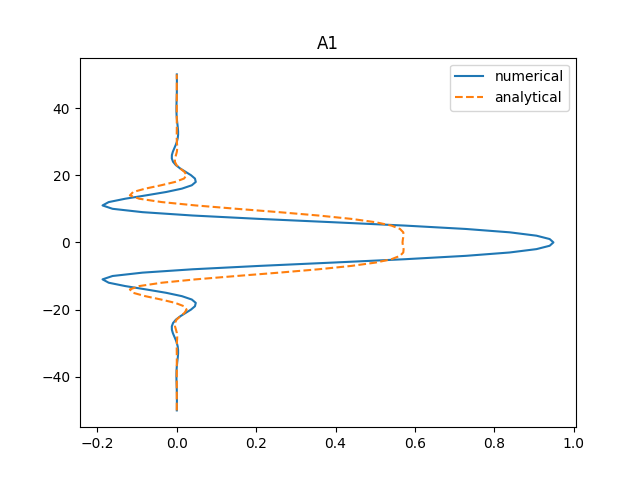
\includegraphics[width = 0.7\textwidth]{../plots/lineA1-compare.png}} \\
\subfloat[x=5]{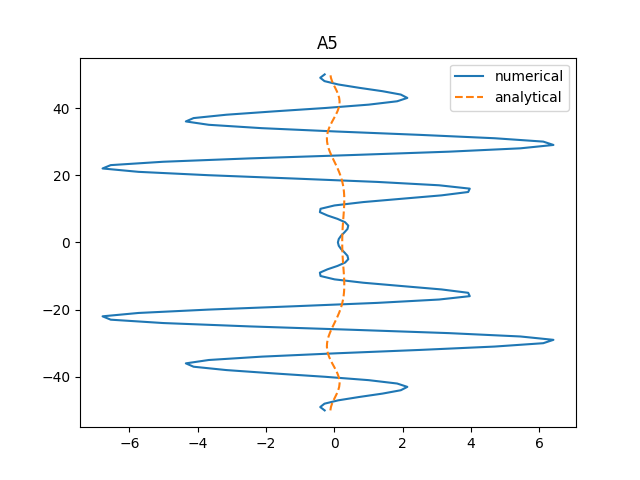
\includegraphics[width = 0.7\textwidth]{../plots/lineA5-compare.png}}
\subfloat[x=6]{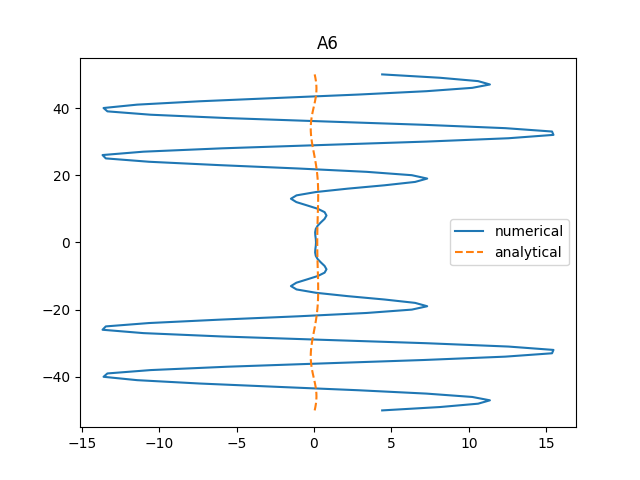
\includegraphics[width = 0.7\textwidth]{../plots/lineA6-compare.png}} \\
\subfloat[x=8]{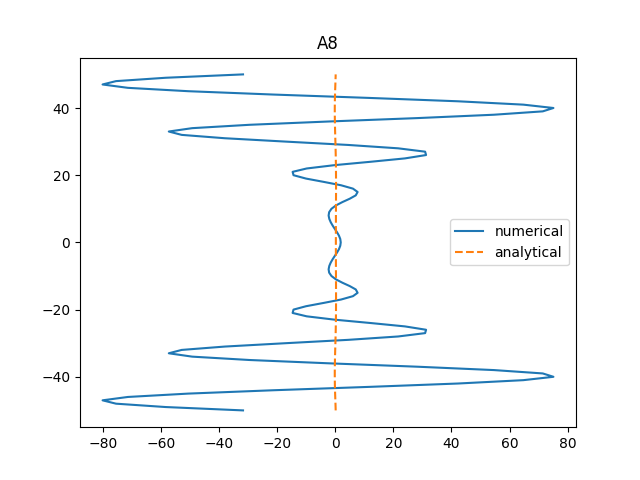
\includegraphics[width = 0.7\textwidth]{../plots/lineA8-compare.png}}
\subfloat[x=20]{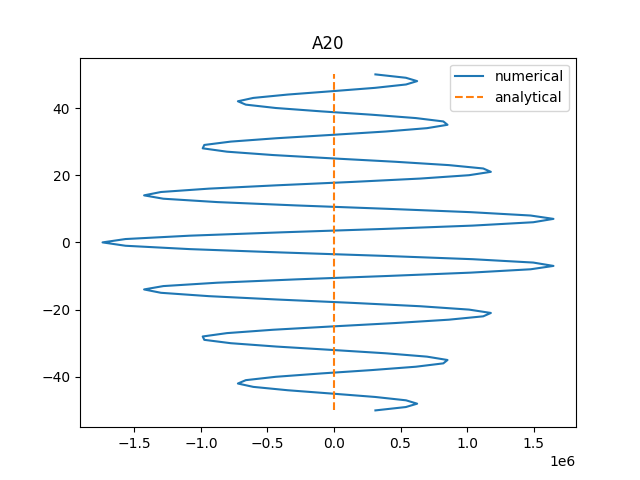
\includegraphics[width = 0.7\textwidth]{../plots/lineA20-compare.png}}
\caption{x-th column of matrix A (numerical) and $\tilde{A}$ (analytical)}
\label{some example}
\end{figure}



\newpage

\subsection{Compare numerical and analytical - decibels}

Functon for converting to decibels:
\begin{python}
''' Function takes a vector (matrix row) and transfores the quantity to decibels '''
def convert_to_decibel(x):
    a0 = x[0]
    new = []
    for i in x:
        if cmath.log10(i/a0) == 0:
            new = new + [1]
        else:
            new = new +  [20*cmath.log10(i/a0)]
    return new
\end{python}


\begin{figure}[H]
\subfloat[x=1]{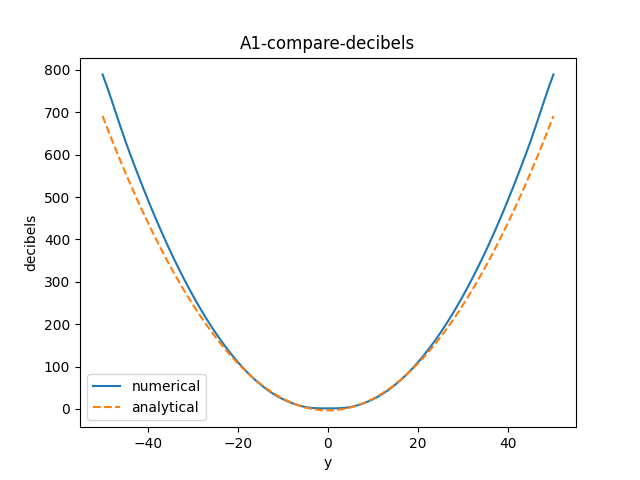
\includegraphics[width = 0.7\textwidth]{../plots/A1-compare-decibels.png}}
\subfloat[x=2]{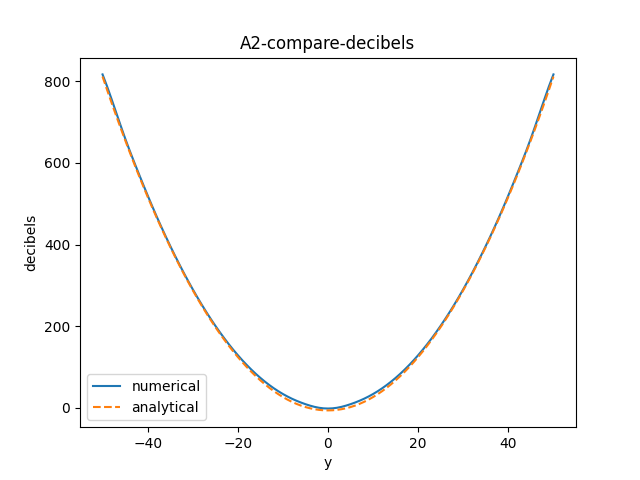
\includegraphics[width = 0.7\textwidth]{../plots/A2-compare-decibels.png}} \\
\subfloat[x=3]{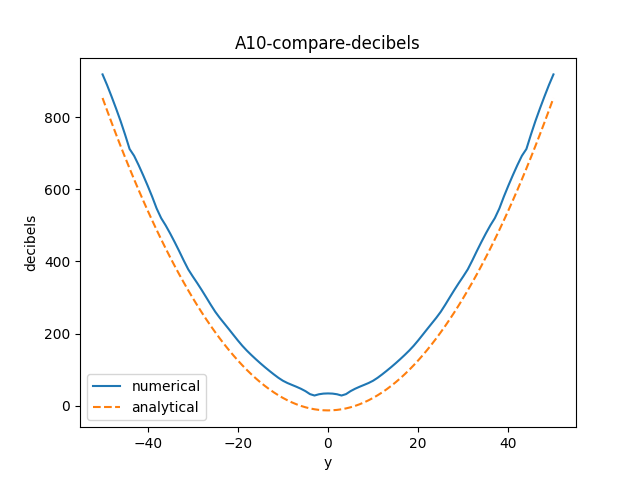
\includegraphics[width = 0.7\textwidth]{../plots/A10-compare-decibels.png}} 
\subfloat[x = 20]{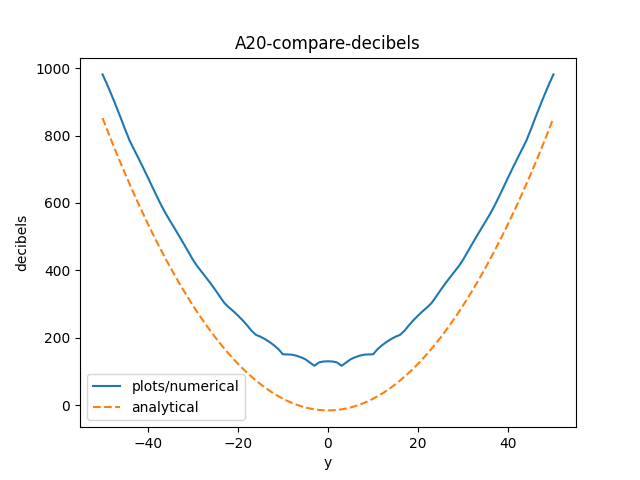
\includegraphics[width = 0.7\textwidth]{../plots/A20-compare-decibels.png}}
\caption{x-th column of matrix A (numerical) and $\tilde{A}$ (analytical) converted to decibels}
\label{some example1}
\end{figure}




\section{$x \in [0 1000], hx = 5 and y \in [-500, 500], hy = 1$}

\subsection{Heatmap}

\begin{figure}[H]
\subfloat[0-3]{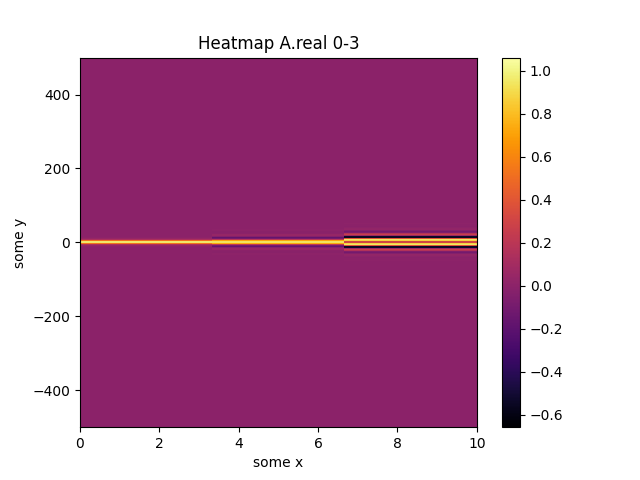
\includegraphics[width = 0.7\textwidth]{../plots/heatmap0-3-bigger.png}}
\subfloat[0-5]{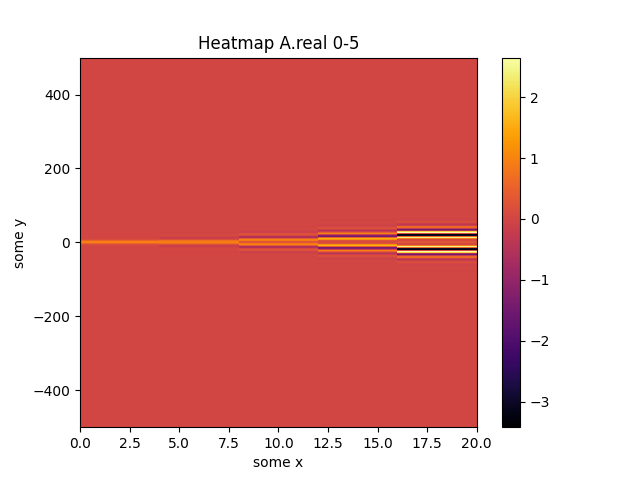
\includegraphics[width = 0.7\textwidth]{../plots/heatmap0-5-bigger.png}} \\
\subfloat[0-10]{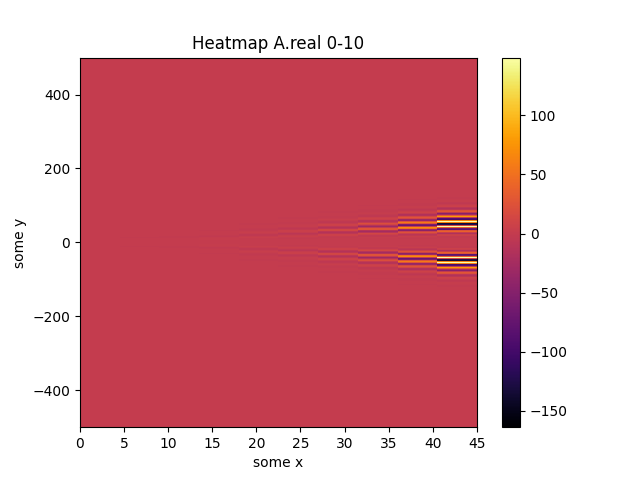
\includegraphics[width = 0.7\textwidth]{../plots/heatmap0-10-bigger.png}}
\subfloat[0-20]{{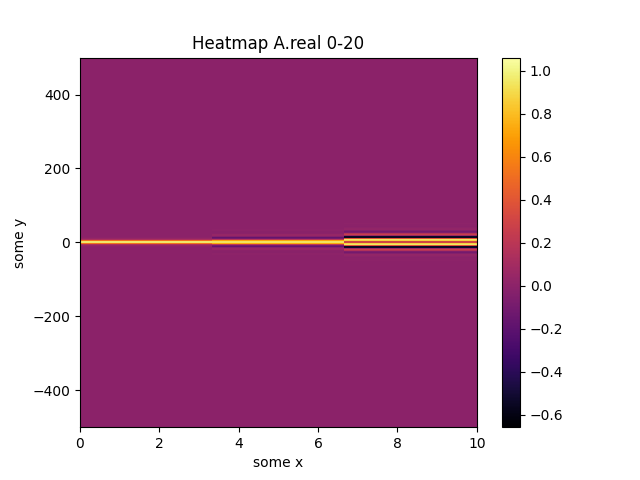
\includegraphics[width = 0.7\textwidth]{../plots/heatmap0-20-bigger.png}}
}
\caption{Heatmap for first n x numerically calculated}
\label{some example3}
\end{figure}



    \begin{figure}[!h]
        \makebox[\textwidth]{
        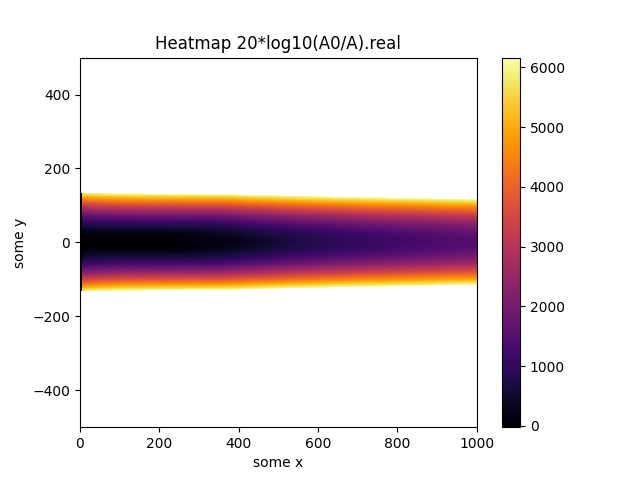
\includegraphics[width = 0.7\textwidth]{../plots/decibels-bigger.png}}
¸    \caption{numerical solution}
        \label{fig: napaka}
    \end{figure}


    \begin{figure}[!h]
        \makebox[\textwidth]{
        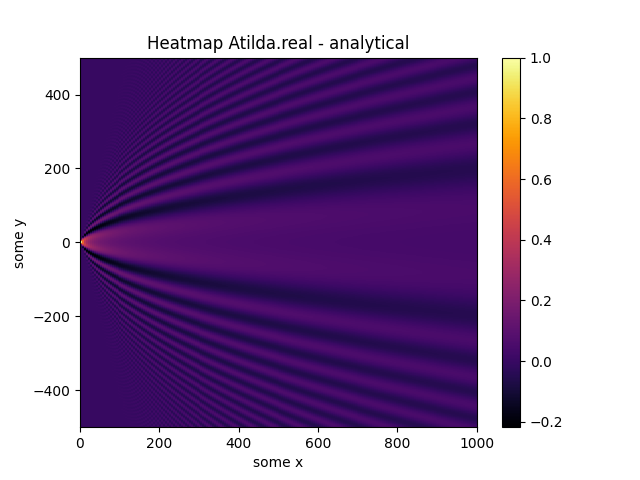
\includegraphics[width = 0.7\textwidth]{../plots/heatmap_tilda-bigger.png}}
¸    \caption{analytical solution}
        \label{fig: heatana}
    \end{figure}

\newpage

\subsection{Compare numerical and analytical}


\begin{figure}[H]
\subfloat[x=0]{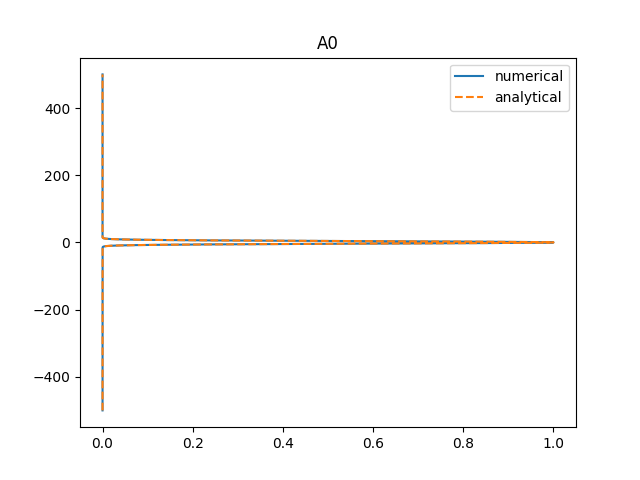
\includegraphics[width = 0.7\textwidth]{../plots/lineA0a-compare-bigger.png}}
\subfloat[x=1]{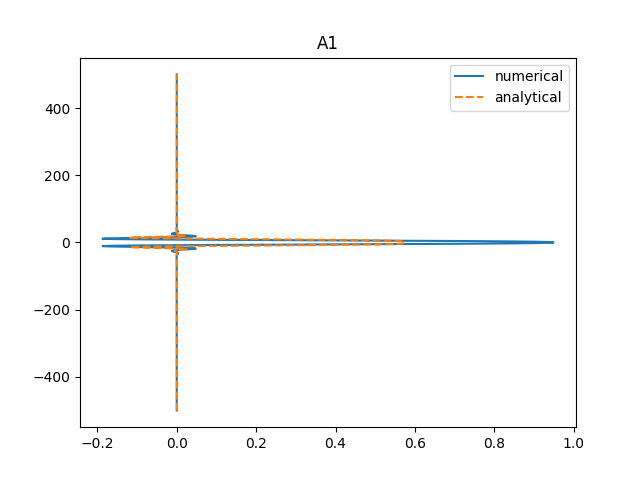
\includegraphics[width = 0.7\textwidth]{../plots/lineA1-compare-bigger.png}} \\
\subfloat[x=5]{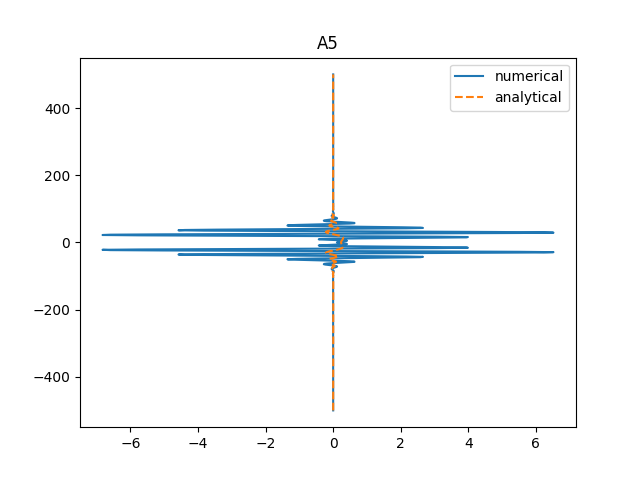
\includegraphics[width = 0.7\textwidth]{../plots/lineA5-compare-bigger.png}}
\subfloat[x=6]{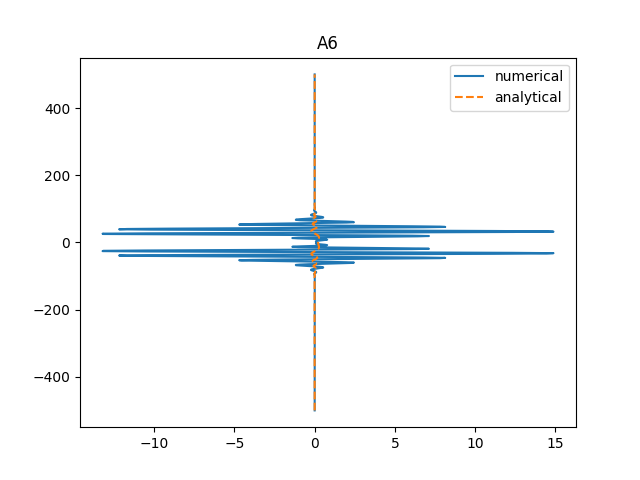
\includegraphics[width = 0.7\textwidth]{../plots/lineA6-compare-bigger.png}} \\
\subfloat[x=8]{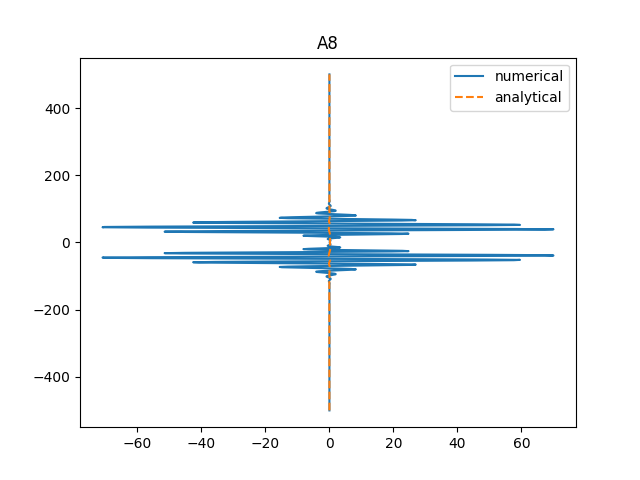
\includegraphics[width = 0.7\textwidth]{../plots/lineA8-compare-bigger.png}}
\subfloat[x=20]{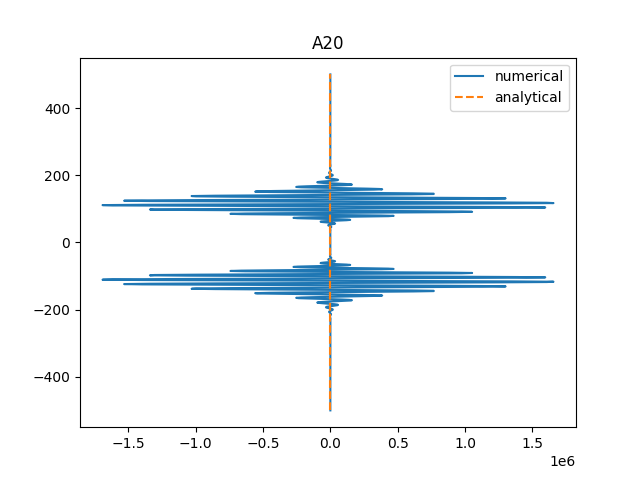
\includegraphics[width = 0.7\textwidth]{../plots/lineA20-compare-bigger.png}}
\caption{x-th column of matrix A (numerical) and $\tilde{A}$ (analytical)}
\label{some example}
\end{figure}



\newpage

\subsection{Compare numerical and analytical - decibels}

Functon for converting to decibels:
\begin{python}
''' Function takes a vector (matrix row) and transfores the quantity to decibels '''
def convert_to_decibel(x):
    a0 = x[0]
    new = []
    for i in x:
        if cmath.log10(i/a0) == 0:
            new = new + [1]
        else:
            new = new +  [20*cmath.log10(i/a0)]
    return new
\end{python}


\begin{figure}[H]
\subfloat[x=1]{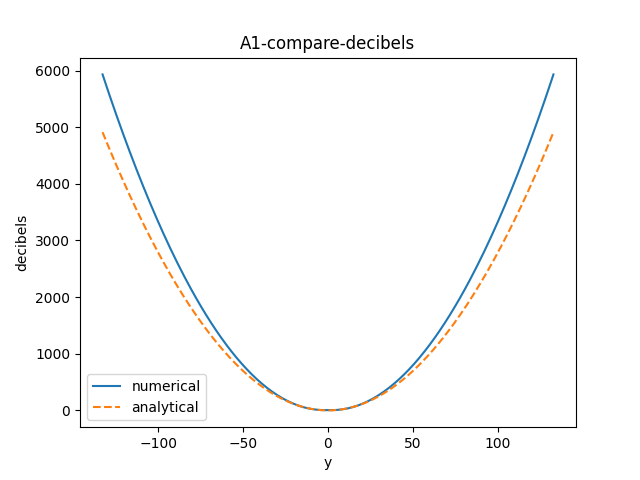
\includegraphics[width = 0.7\textwidth]{../plots/A1-compare-decibels-bigger.png}}
\subfloat[x=2]{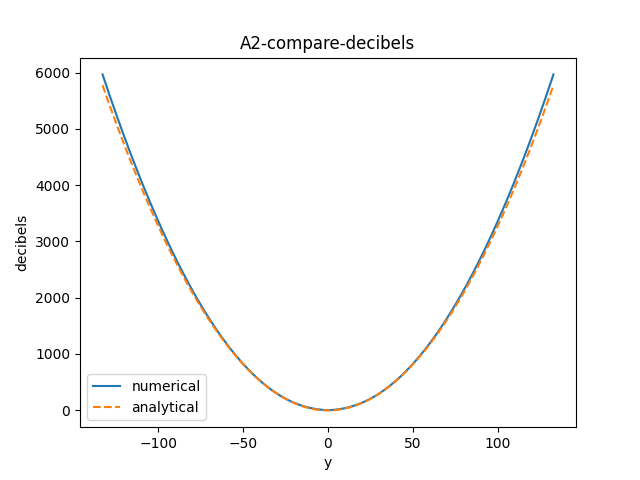
\includegraphics[width = 0.7\textwidth]{../plots/A2-compare-decibels-bigger.png}} \\
\subfloat[x=3]{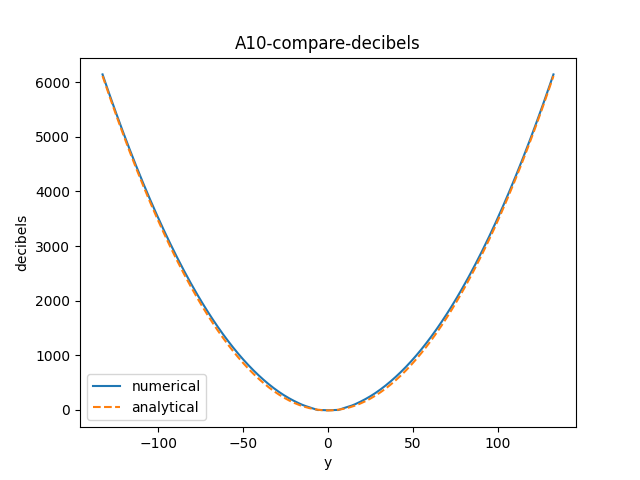
\includegraphics[width = 0.7\textwidth]{../plots/A10-compare-decibels-bigger.png}} 
\subfloat[x = 20]{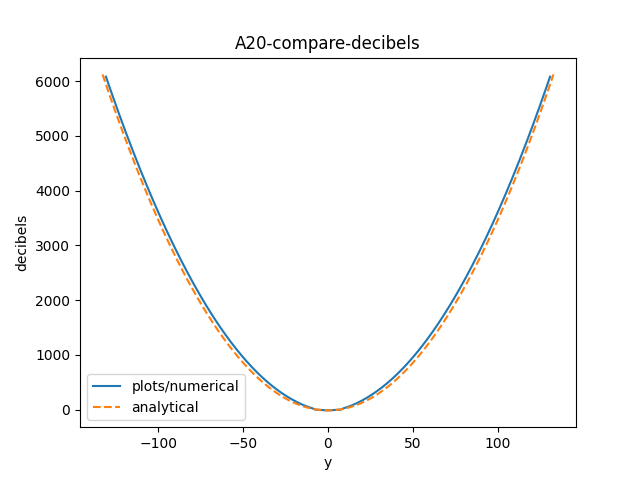
\includegraphics[width = 0.7\textwidth]{../plots/A20-compare-decibels-bigger.png}}
\caption{x-th column of matrix A (numerical) and $\tilde{A}$ (analytical) converted to decibels}
\label{some example1}
\end{figure}


\end{document}